\chapter{Dostupné technologie NFV a VNF}

V předchozí sekci byla popsána myšlenka a motivace související s virtualizací síťových funkcí. V této kapitole bude probrána architektura pro NFV a následně možnosti pro implementaci jednotlivých částí této architektury. 

\section{Architektura NFV a VNF} 

V \cite{NFV_architektura} je popsána referenční architektura pro NFV, která byla navržena organizací ETSI. Jedná se pouze o funkční návrh bez náznaků konkrétní implementace. Obrázek č. \ref{fig:NFV_architektura} znázorňuje tuto architekturu.  

\begin{figure}[h]
\begin{centering}
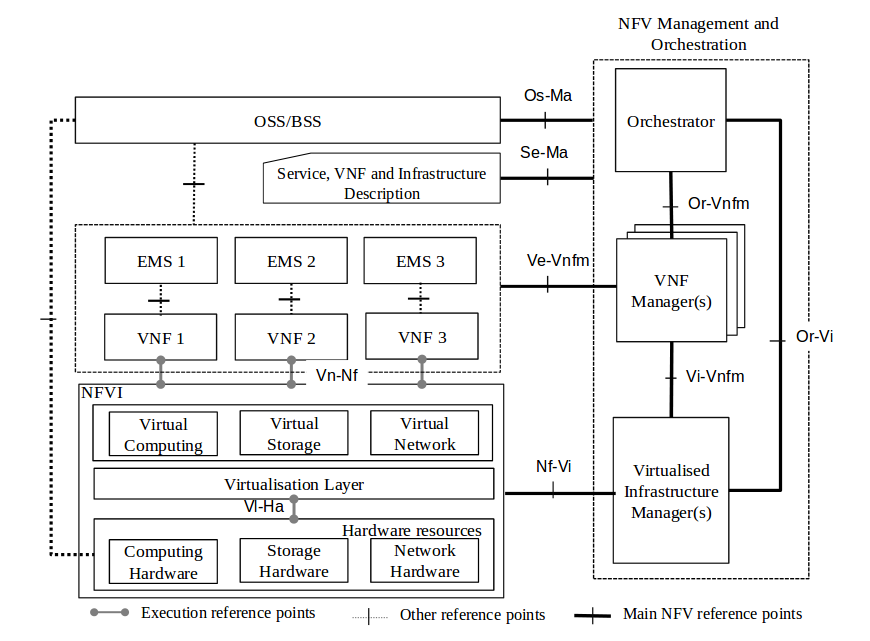
\includegraphics[scale=0.5]{images/NFV_architektura}
\par\end{centering}
\caption{NFV architektura, převzato z \cite{NFV_architektura}\label{fig:NFV_architektura}}
\end{figure}

Z obrázku je patrné, že celá architektura se dá rozdělit na tyto 3 hlavní části, které mezi sebou mají komunikovat. Tyto části jsou:

\begin{itemize}
\item Infrastruktura virtualizace síťových funkcí (NFVI) - Jsou všechny softwarové a hardwarové zdroje potřebné k vytvoření prostředí, ve které mohou být jednotlivé VNF být nasazeny. Tato infrastruktura může být velice rozsáhlá, proto je její součástí i síť poskytující konektivitu mezi vzdálenými lokacemi infrastruktury.
\item Virtualizované síťové funkce (VNFs) - Jsou softwarové implementace síťových funkcí, jako je např. NAT a routing. které mohou být nasazeny na NFV infrastruktuře.
\item Management a orchestrace NFV (NFV-MANO) - zde se jedná o řízení softwarových a hardwarových zdrojů v celé infrastruktuře NFV a životního cyklu jednotlivých virtuálních síťových funkcí. Tato část se tedy zaměřuje na řízení a správu všech úloh související v virtualizací v NFV frameworku.
\end{itemize}

Podrobné vysvětlení všech zkratek a teminologii, která je vyobrazena na obrázku lze nalézt v \cite{NFV_terminology}. Pro účely této práce jsou dále popsány pouze výše uvedené hlavní části architektury.

\subsection{Infrastruktura NFV}

Ve zdroji \cite{NFV_infrastructure}, který detailně popisuje infrastrukturu pro virtualizaci síťových funkcí (NFVI), je uvedeno, že je v ní sdružení všech základních zdrojů potřebných pro běh virtuálních síťových funkcí (VNF). Z tohoto důvodu sem patří veškerý hardware. Do NFVI také patří některé softwarové komponenty, které jsou společné pro mnoho VNF a poskytují funkcionalitu potřebnou pro podporu nasazení, propojení či managementu VNF. Celou infrastrukturu může tvořit jeden či více strojů, které mají tyto potřebné funkce. Tyto stroje také mohou být umístěny v různých spolu spojených geografických lokacích. 

Pro zjednodušení lze celou NFV infrastrukturu rozdělit do 3 následujících domén:

\begin{itemize}
\item Compute Domain - Do této domény patří veškeré hardwarové zdroje jako jsou servery, úložiště a komponenty, které tyto zdroje obsahují, např. procesory, pevné disky, síťové karty, atd. Zároveň je zde řešen návrh fyzické topologie. \cite{NFV_compute}
\item Hypervisor Domain - Toto je doména, které představuje softwarové prostředí abstrahující hardware v compute doméně a poskytuje je jako virtuální zdroje. Tyto zdroje následně mohou využívat virtuální síťové funkce. \cite{NFV_hypervisor}
\item Infrastructure Network Domain - V této doméně je řešeno veškeré propojení výše zmíněných domén. Tedy fyzické i virtuální infrastruktury.\cite{NFV_network}
\end{itemize}

Funkci obsaženou v jednotlivých doménách znázorňuje obrázek č. \ref{fig:infrastruktura}. Více informací na tuto problematiku lze nalézt v \cite{NFV_infrastructure} a ve zdrojích uvedených u každé domény. 

\begin{figure}[h]
\begin{centering}
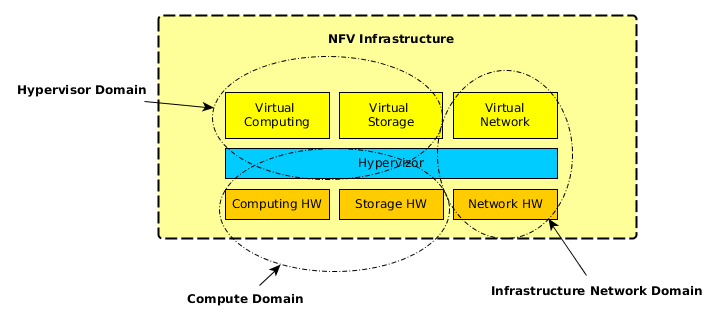
\includegraphics[scale=0.65]{images/infrastruktura}
\par\end{centering}
\caption{Schéma NFV infrastruktury\label{fig:infrastruktura}}
\end{figure}

Dá se říci, že referenční návrh infrastruktury pro NFV je podobný jako pro návrh infrastruktury pro cloud computing platformu. V kapitole \ref{sec:NFVI} jsou uvedeny příklady možných cloudových platforem, které lze NFVI využít.

\subsection{Virtuální síťová funkce}

Virtuální síťová funkce (VNF) je dle \cite{NFV_VNF} určitá síťová funkce, která běží na NVF infrastruktuře a je zároveň NFV frameworkem řízena a spravována. Zároveň musí mít dobře definované rozhraní k ostatním síťovým funkcím, k VNF Managerovi a měla by obsahovat management rozhraní či port. Jedna VNF může být být obsažena v jednom virtuálním stroji nebo může být roztažena přes více virtuálních strojů. 

Na obrázku č. \ref{fig:VNF} je vidět jednoduché schéma virtuální síťové funkce dle referenčního návrhu \cite{NFV_VNF}. Celý životní cyklus VNF (vytvoření, spuštění, zastavení, smazání a škálování) řídí VNF Manager, který je součástí NVF managementu a orchestrace. Současně je možné dynamicky změnit aktuální konfiguraci pomocí Entity manageru (EM) přes management interface. EM může spravovat více VNF nebo právě jednu. Vnitřní struktura celé instance může být tvořena více komponentami (VNFC), které spolu mohou být navzájem provázány. Toto provázání však nemusí být viditelné zvenčí.

\begin{figure}[h]
\begin{centering}
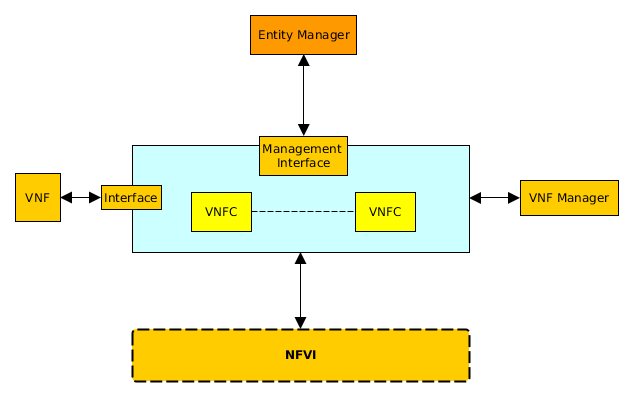
\includegraphics[scale=0.67]{images/VNF}
\par\end{centering}
\caption{Schéma virtuální síťové funkce\label{fig:VNF}}
\end{figure}

Pohledem na současný trh zjistíme, že VNF je prakticky poskytována ve 3 základních podobách.

\begin{itemize}
\item Softwarová aplikace - V tomto případě je poskytována VNF jako aplikace, která může být nainstalována na běžný operační systém jako je například GNU/Linux.
\item Ucelený operační systém - Zde je poskytován přímo celý operační systém, který může být nainstalován do virtuálního stroje nebo i na fyzický server.
\item Kompletní VM - Poskytovatel VNF může dát k dispozici rovnou přetvořený obraz virtuálního stroje (image), který může obsahovat operační systém se síťovými funkcemi. Tento systém však nemusí být klasicky dostupný operační systém jako je GNU/Linux či FreeBSD, ale může se jednat o speciálně vytvořený systém od výrobce. Tento způsob budou využívat poskytovatelé, kteří mají proprietární řešení pro síťová řešení jako je například Cisco či Juniper.
\end{itemize}

V kapitole \ref{sec:VNF} jsou uvedeny příklady softwaru existujícím na současném trhu, který lze využít jako VNF.

\subsection{Management a orchestrace NFV}

Management a orchestrace virtualizace síťových funkcí (NFV MANO) je nejdůležitější část celého NFV frameworku. Je tomu tak, protože MANO zajišťuje správné fungování NFV infrastruktury i jednotlivých virtuálních síťových funkcí. MANO také poskytuje funkce nutné pro provisioning VNF a související operace, jako je jejich konfigurace jednotlivých VNF a infrastruktury, na které běží. Zároveň spravuje a řídí životní cyklus fyzických a virtuálních zdrojů, které slouží pro podporu VNF. 

\begin{figure}[h]
\begin{centering}
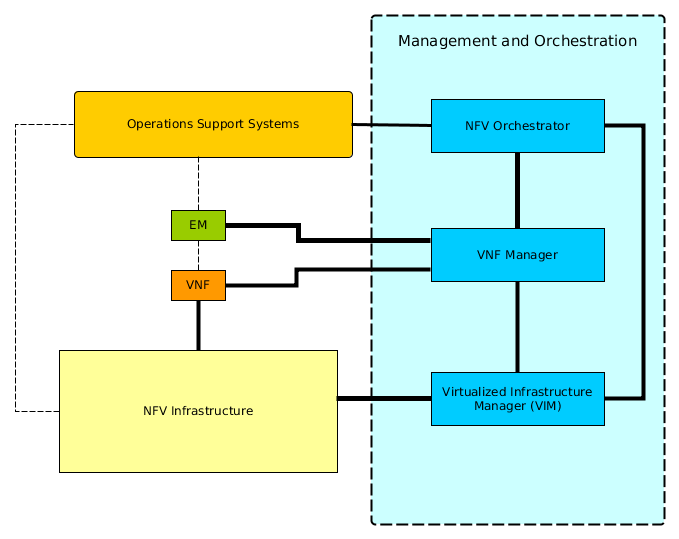
\includegraphics[scale=0.65]{images/MANO}
\par\end{centering}
\caption{Schéma NFV MANO\label{fig:MANO}}
\end{figure}

Jak vyplývá z obrázku č. \ref{fig:MANO}, tak referenční návrh MANO dle \cite{NFV_MANO} se skládá ze hlavních 3 částí, které se zabývají správnou jednotlivých vrstev NFV frameworku.

\begin{itemize}

\item Virtualized infrastructure manager (VIM) - Řídí a spravuje fyzické a virtuální zdroje v jedné doméně infrastuktury. Celková infrastruktura se může skládat z více domén a každá musí mít svůj VIM. Jeho typickými úlohami jsou vytváření, udržování a uvolňování VM na dostupných zdrojích v doméně. Zároveň musí mít přehled o všech těchto a stavu hardwarových zdrojů.

\item VNF manager - Dohlíží na lifecycle management jednotlivých VNF instancí. To znamená, že výtváří, udržuje a ukončuje VNF instance, které běží na jednotlivých VM (ty však spravuje VIM). Opět může existovat více VNF managerů, kteří mohou spravovat jednu či více VNF.

\item NFV orchestator - Zjednodušeně slouží jako řízení a správu všech VIM a všech VNF managerů. Pomocí komunikace s VIM dokáže spravovat dostupné zdroje a pomocí komunikace s VNF managery dokáže řídit síťové služby. Jeho další funkcí je i přehled všech dostupných VNF, neboli katalog VNF, a registrace nových VNF do tohoto katalogu. Ten je pak dostupný uživatelům.
\end{itemize}

Celý systém je navržen tak, že by měl pracovat společně se stávajícími aplikacemi a systémy, které potencionální uživatelé používají pro provoz své infrastruktury a podnikových procesů (Operation support system).

V oblasti NFV MANO probíhá v součastnosti rozsáhlí vývoj a existuje několik projektů, které se tím zabývají. V článek \cite{NFV_orchestration} je nabídnut zajímavý přehled. V kapitole \ref{sec:MANO} je uveden přehled možných přístupů k managementu a konfiguraci jednotlivých VNF.

\section{Dostupné prostředky pro NFV Infrastrukturu} \label{sec:NFVI}

Pro tvorbu NFV infrastruktury bude v této práci využívána cloudová platforma. V přehledu \cite{Cloud_adoption} , který byl zmíněn v úvodu, je také uvedeno, že mezi nejpoužívanější řešení pro cloud patří OpenStack a řešení od společnosti VMware. Tyto dvě jsou dále popsána podrobněji.

\subsection{OpenStack}

OpenStack \cite{OpenStack_web} je open-source platformou umožňující postavit cloud, který může být nainstalován na běžném hardwaru. Toto řešení má za cíl vytvořit dostupnou cloudovou platformu, která bude splňovat všechny potřeby privátních a veřejných cloudů nezávisle na velikosti řešení.

Celá stavba systému OpenStack se skládá z několika na sobě nezávislých projektů (modulů), které řeší různé oblasti cloudové platformy. Tyto projekty mezi sebou komunikují pomocí otevřených API a mohou být spravovány pomocí dashboardu. Celé administrace OpenStacku může být prováděna přes webově rozhraní, příkazovou řádku či přímo pomocí příkazů zaslaných do API. Celé toto řešení se vyznačuje jednoduchostí implementace, škálovatelností a rychlým vývojem nových vylepšení. Hlavními moduly OpenStacku jsou:

\begin{itemize}
\item Keystone - identifikační služba používaná OpenStackem pro autorizaci a autentizaci. Ověřování probíhá pomocí tokenů. Uživatel přihlášením odesílá žádost na Keystone, který tento modul zpracuje, zjistí pověření a vytvoří token. Vytvořený token je poté odesílán s žádostí do ostatních služeb. Zde dojde ke komparaci tokenu se současnou přístupovou politikou a dojde ke zjištění, zdali má uživatel dostatečná oprávnění pro provedení požadovaného úkonu.
\item Glance - služba umožňující práci s virtuálními diskovými obrazy (imagy). Tyto obrazy mohou být uloženy na mnoha různých místech od lokálních systémových disků až po distribuované souborové systémy, jako je OpenStack Storage.
\item Nova - tento modul poskytuje výpočetní služby. Umožňuje tedy běh několika instancí virtuálních strojů na několika hostitelských strojích, nan kterých je nainstalována služba OpenStack compute. OpenStack podporuje hypervizory KVM, QEMU, VMware ESX, Hyper-V, Xen. 
\item Neutron - je služba pro správu všech síťových aspektů OpenStacku. Jedná se tedy o SDN komponentu. Neutron podporuje možnost rozšíření o tzv. pluginy, které umožňují využívat řešení třetích stran pro síťování.
\item Cinder - poskytuje infrastrukturu pro mapování volumů v OpenStacku.
\item Heat - umožňuje automatizovanou orchestraci virtuálních strojů na základě vytvořených templatů.
\item Horizon - představuje dashboard, který umožňuje cloudovým administrátorům a uživatelům spravovat různé zdroje a služby OpenStacku. Dashboard umožňuje interakci s OpenStackovým kontrolerem prostředníctvím API. 
\end{itemize}


Další informace lze nalést například v \cite{OpenStack}. V této práci jsou vzhledem k NFV infrastruktuře nejzajímavějšími Neutron a Heat moduly.

Heat je projekt, který je určen pro Orchestraci. Má za úkol automatické vytvoření požadovaných resourců (instancí, sítí, atd) podle předdefinovaných scénářů tzv. heat templatů. Obrázek č. \ref{fig:heat_engine} znázorňuje jeho funkci. \cite{HEAT}

\begin{figure}[h]
\begin{centering}
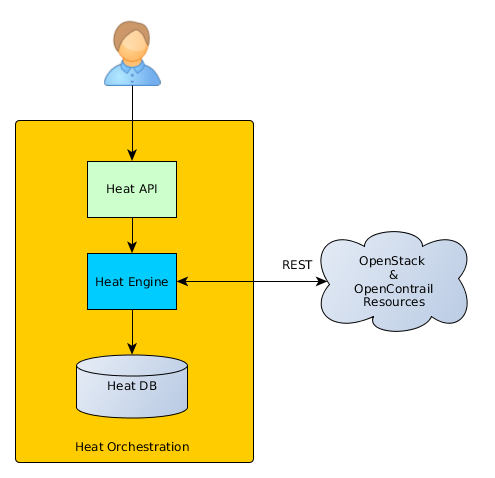
\includegraphics[scale=0.41]{images/heat_engine}
\par\end{centering}
\caption{Popis heat orchestrace\label{fig:heat_engine}}
\end{figure}

Dalším projektem, který v rámci NFV a OpenStacku důležitý je Neutron, který slouží pro práci se sítěmi. Neutron má podporu pro rozšiřující pluginy, které mohou využít SND řešení. Funkce OpenStacku se značně mění dle použitého pluginu, kterých je více než 20. Pokud se podíváme na \cite{neutron_survey} , tak mezi nejpoužívanější patří tzv. Vanilla Neutron a OpenContrail. 

\subsubsection{Vanilla Neutron}

Vanilla Neutron nabízí základní funkcionalitu pro networking v prostředí OpenStack, kterou uživatel může vyžadovat. Je to z důvodů toho, že OpenStack původně vyšel z AWS (Amazon Web Services) a jeho cílem bylo sjednotit privátní a veřejný cloud. Dnes do Neutronu přibývají další funkce jako je například VPNaaS.

Problém samotného Neutronu je, že prozatím nemá podporu pro NFV. Proto byla vytvorena iniciativa OP-NFV \cite{opnfv} , která se snaží vytvořit otevřený framework pro NFV založený na OpenStacku. Přestože tento projekt má velký potenciál, tak v době psaní této práce je v začátcích a není vhodný pro produkční nasazení.

\subsubsection{OpenContrail} 

OpenContrail je jeden z nejpoužívanějších komerčně dostupných řešení pro networking pro OpenStack. Obsahuje všechny potřebné komponenty pro virtualizaci síťí v cloudovém prostředí - SND controller, virtuální router, analytický engine a REST API. \cite{OpenContrail}

OpenContrail není pouze SDN řešení, ale je to i řešení pro NFV. OpenContrail obsahuje funkci Service Chainingu. Tím pádem umožňuje dynamicky vytváření instancí, které mohou sloužit jako VNF. Zároveň také dokáže řídit datový tok z ostatních instancí resp. virtuálních sítí k nimž je VNF připojena tak, aby procházela právě danou VNF. V poslední verzi dále přínáší nové funkce jako BGPaaS a Physical Service Chaining. Je to tedy komplexní řešení vhodné pro produkční nasazování. 

\subsection{VMware vCloud Suite}

Společnost VMware \cite{vmware_web} se původně zabývala vývojem předního virtualizačního nástroje. Postupně nabrala do svého portfolia i další služby a rozšířila působnost obecně na virtualizaci a služby s ní úzce spojené. Mezi ně dnes patří i cloudová platforma. 

VMware vCloud Suite je právě určený pro vytváření privátních cloudů. Je to řešení poskládané z jednotlivých prodůktů společnosti VMware. Jeho hlavními komponentami jsou:

\begin{itemize}
\item VMware vCloud Director - je  jedna  ze základních součástí potřebných pro vytvoření  privátního  cloudu ve stylu VMwaru.  Umožňuje vytvořit  a  doručovat  koncovým  zákazníkům infrastrukturu jako službu. Je propojen a přímo spolupracuje s VMware vSphere center.
\item VMware vSphere - tento produkt slouží pro vytvoření virtualizované infrastruktury. Je to sdružení více komponent. Ty nejhlavnější jsou:
\begin{itemize}
\item VMware ESX (ESXi) - je to bare-metal hypevizor.
\item VMware vCenter Server - umožňuje efektivní a pokročilejčí správu virtualizovaného prostředí, bez ohledu na jeho velikost. Jedná se např.o snadné vytváření nových virtuálních počítačů, jejich  klonování  nebo  importování  z jiného  úložiště.  
\item VMware vSphere Client - je určený pro dálkovou správu hostitelů ESXi. Připojit se můžeme prostřednictvím vCenter serveru nebo přímo přes ESXi server.
\end{itemize} 
\item VMware vCloud Networking and Security - poskytuje síťování a bezpečnost pro vituální prostředí. Poskytuje mnoho síťových funkcí a poskytuje framework pro integraci řešeí třetích stran.
\item VMware vShield - představuje možnost zabezpečení v prostředí VMware VSphere. Může být konfigurován pomocí vShield Managera, který umožňuje centrální správu přes webové rozhraní, vSphere klient plug-in, nebo command line interface (CLI).
\item VMware vCenter Chargeback - slouží pro monitorování virtuálních strojů, které následně může být účtováno.
\end{itemize}

VMware VCloud Suite má hierarchickou strukturu, kterou znázorňuje obrázek č. \ref{fig:vmware}. Více informací o tomto řešení čí jeho částech nabízí např. \cite{vmware} .

\begin{figure}[h]
\begin{centering}
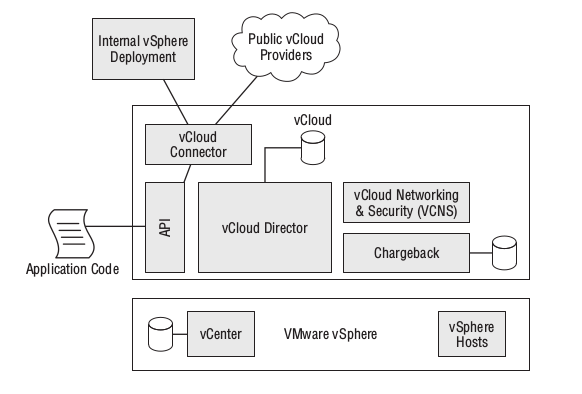
\includegraphics[scale=0.65]{images/vmware}
\par\end{centering}
\caption{Schéma VMware vCloud Suite, převzato z \cite{vmware_obrazek}\label{fig:vmware}}
\end{figure}

Celé vmware řešení je proprietární. To znamená, že kód pro jednotlivé komponenty je uzavřený a není do něj přístup. S tím zamozřejmě souvisí i licence. Pro používání jakéhokoli produktu od společnosti VMware v produkčním prostředí je potřeba zakoupení licence. Všechny produkty této společnosti se vyznačují tím, že je vše ovládané z grafického uživatelského prostředí bez nutonosti použití příkazové řádky. Je však toto řešení dostatečně standartní pro NFV Infrastrukturu?

Pokud se podíváme na možnosti orchestrace, tak je zde oproti předchozímu řešení zvolený odlišný přístup. Přestože VMware poskytuje REST API, tak vše je orientované na ovládání zkrze dashboard. To znamená, že automatizace či předdefinování scénářu pro vytváření resourců zde spočívá v naklikání celého workflow v přehledném GUI.

Pro networking v této cloudové platformě existuje tzv. VMware NSX. Je to SDN Controller, které je opět velmi často používané i s cloudovou plaformou OpenStack. Přestože opět obsahuje vše potřebné pro vytváření a správu virtuálních sítí, tak zde není přímá podpora NFV, která by usnadnila práci s jednotlivými VNF.


\section{Dostupné možnosti pro VNF} \label{sec:VNF}

Protože v této práci mají být ukázány příklady pro vytváření a management VNF. Je nutné najít software, který může být použit jako VNF. Protože exituje celá řada síťových funkcí a bylo by nad rámec této práce zmínit všechna jejich řešení, tak bylo nutné výběr zúžit výběr na dvě nejčastěji používané síťové funkce. Těmi jsou firewall a load balancer. Dále je tedy uveden software, který je možné použít pro Firewall as a Service (FwaaS) a Load balancer as a Service (LbaaS).

\subsection{Firewall as a Service}

Pokud se podíváme na vendory ve zdroji \cite{firewalls} , jejichž firewally jsou nejvíce využívány, tak zjistíme, že mnozí již chápou důležitost NFV a své produkty začínají poskytovat jako virtuální instance, které se dají použít pro účely VNF v této práci. Jedná se například o tyto:

\begin{itemize}
\item Fortigate-VM - Fortigate Virtual Appliances je řešení pro cloudové prostředí od společnosti Fortinet. Nabízí stejně funkce pro firewall jako jsou obsaženy ve Fortigate fyzických zařízeních. \cite{fortigate}
\item Juniper vSRX - Jde o firewall od společnosti Juniper, který je obdobou jejich fyzického zařízení Juniper SRX. Jde virtuální instanci poskytující funkce pro firewall, routing a pokročilé bezpečností funkce pro poskytovale telekomunikačních služeb a větší společnosti. Toto VM je určené pro privátní, public i hybrid cloud. \cite{juniper}
\item Cisco virtual ASA - Společnost Cisco nabízí Adaptive Security Virtual Appliance (ASAv), která obsahuje stejný software jako fyzické ASA zařízení a vetšinu funkcí pro firewall, routing a VPN. \cite{cisco}
\item PFSense - PFSense je open-source projekt, který má za cíl poskytnout firewall postavený na operačním systému FreeBSD, který může běžet na klasické architektuře jednodeskových počítaču. Toto řešení poskytuje všechny důležité vlastnosti komerčních firewallů, má jednoduché ovládání a je to otevřené řešení. \cite{pfsense}
\end{itemize} 

\subsection{Load balancer as a Service}

Na trhu s virtuálními load balancery je situace podobná. Zde vendoři také začínají poskytovat virtuální instance či software. Pro správné fungování load balancu je však nejlepší, pokud existuje integrace či plugin pro danou cloudovou platformu či používané SDN. Výše zmíněný VMware i OpenStack podporují následující software sloužící jako LbaaS.

\begin{itemize}
\item HAproxy – Je velmi rychlé a spolehlivé řešení nabízející vysokou dostupnost, load balancing a proxy pro aplikace založené na TCP a HTTP. Jedná se de-facto o standartní opensource load balancer, který občas býcá součástní některých linuxových distibucí. Velice oblíbené je jeho využítí práce cloudových platformách, kde je jako defaultní možnost pro load balancing. Více informací poskytuje \cite{HAproxy} .
\item AVI networks - Je celkem nová společnost poskytující platformu, která poskytuje automatizované aplikační služby zahrnující load balancing, aplikační analýzu a prediktivní auto škálování. Platforma je postavena na softwarově definovaném pricipu a tím pádem může být nasazena klasickou x86 platformu serverů. Více informací obsahuje \cite{avi_networks} .
\end{itemize}

\section{Možnosti prostředky pro Management a Orchestraci VNF} \label{sec:MANO}

Poslední částí refenční architektury NFV je management a orchestrace VNF. Přestože se jedná o nejkomplexnější část architektury, tak v této práci se situace o něco zjednodušila použitím cloudové platformy. Díky ní totiž není nutné hledat řešení pro úlohu, kterou plní Virtualized infrastructure manager, neboť pokuď bude provedena správná volba této platformy, tak v ní bude již obsažena. Zároveň je třeba říci, že zde Není tedy nutné se příliš starat o to, kde budou jednotlivá VNF vytvořena, přestože z hlediska výkonu to může hrát roli, jak je například popsáno v \cite{vnf_placement} .

Dále je nutné zmínit, že není nutné realizovat roli NFV orchestatoru, protože by to bylo nad rámec cílů této práce. Jediným problémem, pro který je tedy nutné navrhnout řešení je management jednotlivých síťových funkcí. Roli, kterou zastává VNF manager. Tou je tedy management jednotlivých VNF a softwaru, který na nich poběží.

Management počítačové sítě je sama osobě komplexní činnost skládající dle \cite{network_management} se ze:

\begin{itemize}
\item Správa poruch a chyb (ang. Fault management)
\item Správa konfigurace (ang. Configuration management)
\item Účetní a evidenční správa (ang. Accounting management)
\item Správa výkonu (ang. Performance management) 
\item Správa bezpečnosti (ang. Security management)
\end{itemize}

Přestože všechny tyto části jsou důležité, tak kromě správy konfigurace jsou to detekční a monitorovací úkony, které mohou být do určité míry i součástí implementace cloudové platformy. Avšak správa konfigurace je hlavní část, pro kterou je nutné nalést řešení v této práci, protože většina softwaru pro VNF uvedené v předchozí části bude mít jiné možnosti pro jejich správu konfigurace. Existuje zde tedy několik přístupů, jak k ní přistupovat. Některé jsou zmíněné v předchozí práci \cite{bakalarka}. Pro účely této práce lze uvažovat o následujících:

\begin{itemize}
\item Předdefinovaný image či aplikace - V tomto případě je veškerá potřebná konfigurace součástí dodávaného image. Pokud je požadována jednoduchá síťová funkce, jejíž konfigurace se v čase nebude měnit, pak je toto nejlepší způsob.
\item Využití scriptování / API - Pokud daná VNF poskytuje API či podporuje skriptovací rozhraní, pak je možné ho využít a dopravit, tak požadovanou konfiguraci.
\item Standardizované protokoly - Dnes již také existují relativně standardizované protokoli určené právě pro správu konfigurace. Jedním je například protokol NETCONF, jak je uvedeno v \cite{network_management}
\item Konfigurační management - Další možností je využití konfiguračního managementu, který se dnes velmi často využívá při správě velkého množství serverů. Zde je však nutné, aby daná VNF podporovala danou metodu správy, kterou využívají jednotlivé konfigurační managementy. Může být například vyžadováno, aby daná VNF obsahovala agenta, který bude pro konfiguraci využíván. Dnes existuje několik řešení pro konfigurační management jako je např. SaltStack, Puppet či Ansible.
\end{itemize}





